\documentclass[
11pt, % Set the default font size, options include: 8pt, 9pt, 10pt, 11pt, 12pt, 14pt, 17pt, 20pt
%t, % Uncomment to vertically align all slide content to the top of the slide, rather than the default centered
%aspectratio=169, % Uncomment to set the aspect ratio to a 16:9 ratio which matches the aspect ratio of 1080p and 4K screens and projectors
]{beamer}

\graphicspath{{Images/}{./}} % Specifies where to look for included images (trailing slash required)

\usepackage{todonotes}
\usepackage{graphicx}
\usepackage{xcolor}
\usepackage{subfig}
%%\usepackage[noend]{algpseudocode}

%
%\usepackage{algorithm}
%\usepackage{algorithmic}
\usepackage{algorithm}
\usepackage{algpseudocode}
\usepackage{blkarray}
\usepackage{amsmath}
\usepackage{xspace}
\usepackage{float}


\usepackage{tikz}
\usetikzlibrary{matrix, decorations, patterns, positioning, shapes, calc, intersections, arrows, fit}

\usetikzlibrary{patterns}
\usetikzlibrary{fit,calc,positioning,decorations.pathreplacing,matrix,3d, hobby}

\usepackage{booktabs} % Allows the use of \toprule, \midrule and \bottomrule for better rules in tables
\usepackage{bm}
\usepackage{multirow}

\newcommand{\brown}[1]{{\color{brown} #1 }}

%% Colors from https://latexcolor.com/
\definecolor{pastelviolet}{rgb}{0.8, 0.6, 0.79}
\definecolor{babyblueeyes}{rgb}{0.63, 0.79, 0.95}
\definecolor{pastelyellow}{rgb}{0.99, 0.99, 0.59}
\definecolor{pastelgreen}{rgb}{0.47, 0.87, 0.47}
\definecolor{pastelred}{rgb}{1.0, 0.41, 0.38}
\colorlet{patternblue}{blue!60}


\colorlet{darkred}{red!80!black}
\colorlet{darkblue}{blue!80!black}
\newcommand<>{\darkred}[1]{{\color{darkred}{#1}}}
\newcommand<>{\darkblue}[1]{{\color#2{blue!50!black!100}{#1}}}

\newcommand{\A}{\mathbf{A}}
\newcommand{\B}{\mathbf{B}}
\newcommand{\CC}{\mathbf{C}}
\newcommand{\Real}{\mathbb{R}}
\newcommand{\vc}[1]{\bm{#1}}

\usetheme{Madrid}

\newcommand{\Tra}{{\sf T}} 


\newcommand{\Ms}[2]{\mathbf{#1}^{(#2)}} 
\newcommand{\M}[1]{\mathbf{#1}} 
\newcommand{\Mb}[2]{\mathbf{#1}_{#2}} 
\newcommand{\Mbs}[3]{\mathbf{#1}_{#2}^{(#3)}} 

%\usepackage{enumitem}



%----------------------------------------------------------------------------------------
%	PRESENTATION INFORMATION
%----------------------------------------------------------------------------------------

\title[Symmetric computations]{Symmetric computations} % The short title in the optional parameter appears at the bottom of every slide, the full title in the main parameter is only on the title page

%\subtitle{Optional Subtitle} % Presentation subtitle, remove this command if a subtitle isn't required

\author[Suraj Kumar]{Suraj Kumar} % Presenter name(s), the optional parameter can contain a shortened version to appear on the bottom of every slide, while the main parameter will appear on the title slide

\institute[Inria \& ENS Lyon]{Inria \& ENS Lyon \\ \smallskip Email:\textit{suraj.kumar@ens-lyon.fr}} % Your institution, the optional parameter can be used for the institution shorthand and will appear on the bottom of every slide after author names, while the required parameter is used on the title slide and can include your email address or additional information on separate lines

\date[CR12]{CR12: September 2024\\ \smallskip\small https://surakuma.github.io/courses/daamtc.html} % Presentation date or conference/meeting name, the optional parameter can contain a shortened version to appear on the bottom of every slide, while the required parameter value is output to the title slide

%----------------------------------------------------------------------------------------

\begin{document}
	
	%----------------------------------------------------------------------------------------
	%	TITLE SLIDE
	%----------------------------------------------------------------------------------------
	
	\begin{frame}
		\titlepage % Output the title slide, automatically created using the text entered in the PRESENTATION INFORMATION block above
	\end{frame}


%	\begin{frame}{Table of Contents}		
%	\tableofcontents[currentsection,hideallsubsections] % Output the table of contents (all sections on one slide)		
%	\end{frame}

\begin{frame}{Symmetric Rank-K (SYRK) update}
	
	\small
	$C=A\cdot A^T$, where $A$ is an $n_1 \times n_2$ matrix and $C$ is an $n_1\times n_1$ symmetric matrix.
\begin{itemize}
	\item It multiplies a matrix with its transpose
	\item It requires roughly half of the computation of general matrix multiplication due to symmetry
	\item $C_{ij} = \sum_{k=0}^{n_2-1}A_{ik}A_{jk}$ for $0\le j \le i \le n_1$
\end{itemize}
\vfill


\begin{minipage}{0.56\linewidth}
SYRK pseudo code:
%	\vspace{-0.45cm}	
	\begin{align*}
	%	&\text{Assuming $C$ is initialized to 0}\\
	&\text{for $i = 0{:}n_1-1$}\\
	&\quad \text{for $j = 0{:}i$}\\
	&\quad\quad \text{for $k = 0{:}n_2-1$}\\
	&\quad\quad\quad C[i][j] += A[i][k]*A[j][k]
	\end{align*}
\end{minipage}
\hfill
\begin{minipage}{0.375\linewidth}
$\qquad$SYRK iteration space:

		\centerline{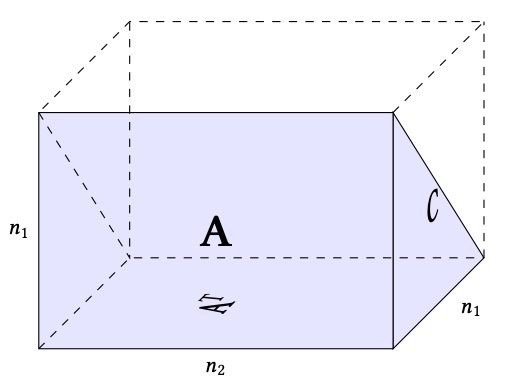
\includegraphics[scale=0.195]{syrkIterationSpace.jpg}}
	
\end{minipage}
\vfill
Here we assume that each $C[i][j]$ is initialized to $0$ in the beginning.
\end{frame}

\begin{frame}{Loomis-Whitney inequalitiy}
\small
	\begin{itemize}
		\item For the $2$d object $G$, $ Area(G) \le \phi_x \phi_y$
		\item For the $3$d object $H$, $Volume(H) \le \sqrt{\phi_{xy}\phi_{yz}\phi_{xz}}$
	\end{itemize}


\begin{center}
	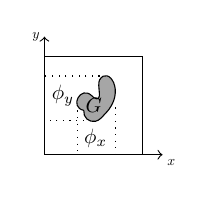
\begin{tikzpicture}[scale=0.25, every node/.style={transform shape}]
	\draw (0,0) -- ++(5,0) -- ++(0, 5) -- ++(-5,0) -- cycle;
	\draw [<->] (0,6) -- (0,0) -- (6,0);
	\node [below right, scale=2] at (6,0) {$x$};
	\node [left, scale=2] at (0,6) {$y$};
	
	\draw [fill=gray!70] (2,2.25) to [curve through={(2.4,3) .. (2.5,2.9) .. (2.8,3.8) .. (3.1,2.1) .. (2.6,1.7)}] (2,2.25);
	
	\node [scale=3] at (2.5,2.5) {$G$};
	\draw [dotted] (1.7,2.25) -- (1.7,0);
	\draw [dotted] (3.6,2.4) -- (3.6,0);
	
	\node[above, scale=3] at (2.6,0) {$\phi_x$};
	
	\draw [dotted] (2,1.75) -- (0,1.75);
	\draw [dotted] (2.8,4) -- (0,4);
	
	\node[right, scale=3] at (0,3) {$\phi_y$};
	\end{tikzpicture}
	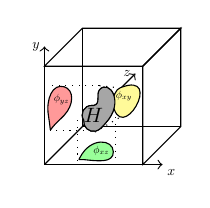
\begin{tikzpicture}[scale=0.25, every node/.style={transform shape}]
	\draw (0,0) -- ++(5,0) -- ++(0, 5) -- ++(-5,0) -- cycle;
	\draw (0,5,0) -- ++(0,0, -5) -- ++(5,0,0) -- ++(0,0,5) -- cycle;
	\draw (5,0,0) -- ++(0,0,-5) -- ++(0,5,0) -- ++(0,0,5) -- cycle;
	\draw (0,0,-5) -- ++(5,0,0) -- ++(0,5,0) -- ++(-5,0,0) -- cycle;
	\draw [<->] (0,6) -- (0,0) -- (6,0);
	\draw [->] (0,0,0) -- (0,0,-12);
	\node [left, scale=2, rotate=0] at (0,0,-12) {$z$};
	\node [below right, scale=2] at (6,0) {$x$};
	\node [left, scale=2] at (0,6) {$y$};
	
	\draw [fill=gray!70] (2,2.25) to [curve through={(2.4,3) .. (2.5,3) .. (2.8,3.8) .. (3.1,2.1) .. (2.6,1.7)}] (2,2.25);
	
	%				\node [scale=2] at (2.5,2.5) {$G$};
	\draw [dotted] (1.7,2.25) -- (1.7,0.2);
	\draw [dotted] (3.6,2.4) -- (3.6,0.3);
	
	\draw [fill=green!40] (1.75,0.25) to [curve through={(1.8, 0.35) .. (3.5, 0.65) .. (2,0.25)}] (1.75,0.25);
	\node[above, scale=1.5] at (2.6,0,-0.75) {$\phi_{xz}$};
	
	\draw [dotted] (2,1.75) -- (0.3,1.75);
	\draw [dotted] (2.8,4) -- (0.385,4);
	
	\draw [fill=red!40] (0.3, 1.75) to [curve through={(0.5,2) .. (1, 2.5) .. (1,3.95) .. (0.2, 2.5)}] (0.3,1.75);
	\node[right, scale=1.5] at (0,3, -0.75) {$\phi_{yz}$};
	
	\draw [fill=yellow!40] (3.85,3.9) to [curve through={(3.7,3.8) .. (3.5,3.4) .. (3.45,3.2)}] (3.85, 3.9);
	\node [scale=1.5] at (3.65,3.1,-1) {$\phi_{xy}$};
	\draw [dotted] (2.8,4) -- (3.8,3.9);
	\draw [dotted] (2.56,1.65) -- (4,2.5);
	
	\draw [fill=gray!70] (2,2.25) to [curve through={(2.4,3) .. (2.5,3) .. (2.8,3.8) .. (3.1,2.1) .. (2.6,1.7)}] (2,2.25);
	
	\node [scale=3] at (2.5,2.5) {$H$};
	\end{tikzpicture}
\end{center}

\vfill
\begin{lemma}
	Let $V\in \mathbb{Z}^3$ and $\phi_{ij}(V)$ be the projection of $V$ on the $i-j$ plane, i.e., $\phi_{ij}(V)= \{(i,j): \exists k, (i,j,k) \in V \}$. Similarly $\phi_{jk}(V)$ and $\phi_{ik}(V)$ are defined. Then $$|V| \le |\phi_{ij}(V)|^\frac12 |\phi_{jk}(V)|^\frac12 |\phi_{ik}(V)|^\frac12\text.$$
\end{lemma}

\end{frame}

\begin{frame}{Extension of Loomis-Whitney inequality}
	\small
\begin{theorem}[Lemma 3, Ballard et al., SPAA 2023.]
	Let $V=\{(i,j,k)\in \mathbb{Z}^3: j < i\}$ and $\phi_{ij}(V)$ be the projection of $V$ on the $i-j$ plane, i.e., $\phi_{ij}(V)= \{(i,j): \exists k, (i,j,k) \in V \}$. Similarly $\phi_{jk}(V)$ and $\phi_{ik}(V)$ are defined. Then $$2|V| \le |\phi_{jk}(V)\cup \phi_{ik}(V)| \left(2|\phi_{ij}(V) |\right)^\frac12 \text.$$
\end{theorem}
\vfill
\begin{minipage}{0.6\linewidth}
Proof: Let $\tilde{V} = \{(i,j,k)\in \mathbb{Z}^3: (j,i,k) \in V\}$.
\begin{itemize}
	\item[] $|V|=|\tilde{V}|$ and $|V\cup\tilde{V}| = 2|V|$
	\item[]  $\phi_{ij}(\tilde{V}) = \{(i,j): (j,i)\in \phi_{ij}(V)\}$ and $|\phi_{ij}(V) \cup \phi_{ij}(\tilde{V})| =  2|\phi_{ij}(V)|$
	\item[]  $\phi_{jk}(\tilde{V}) = \phi_{ik}(V)$, $\phi_{ik}(\tilde{V}) = \phi_{jk}(V)$ and $\phi_{ik}(V\cup\tilde{V}) = \phi_{jk}(V\cup\tilde{V}) = \phi_{jk}(V)\cup \phi_{ik}(V)$
\end{itemize}
\end{minipage}\hfill
\begin{minipage}{0.3\linewidth}
%!TEX root = ../paper.tex

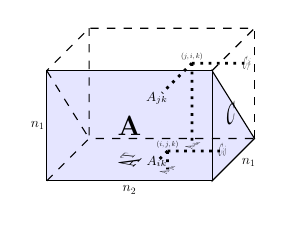
\begin{tikzpicture}[scale=.35,every node/.append style={transform shape}]

% set iteration space dimensions
\pgfmathsetmacro{\idim}{4}
\pgfmathsetmacro{\kdim}{6}

% set internal vertex
\pgfmathsetmacro{\ipt}{1.05*\idim/6}
\pgfmathsetmacro{\jpt}{-\idim/4}
\pgfmathsetmacro{\kpt}{-\kdim/3}

\pgfmathsetmacro{\offset}{.33}

	
% right face of comp cube
\begin{scope}[canvas is yz plane at x=0]
	\draw[black,dashed] (0,-\idim) -- (\idim,-\idim);
	\draw[black,fill=blue!10] (0,0) -- (0,-\idim) -- (\idim,0) -- cycle;
	\node[rotate=-90,scale=2] at (7*\idim/16,-7*\idim/16) {\Large $\CC$};
	\coordinate (c) at (\ipt,\jpt);
	\node[rotate=-90,scale=1.5] at (c) {$C_{ij}$};
	\coordinate (ct) at (\idim+\jpt,-\idim+\ipt);
	\node[rotate=-90,scale=1.5] at (ct) {$C_{ji}$};
\end{scope}
% front face of comp cube
\begin{scope}[canvas is xy plane at z=0]
	\draw[black,fill=blue!10] (0,0) rectangle (-\kdim,\idim);
	\node[scale=2] at (-\kdim/2,\idim/2) {\Large $\A$};
	\node at (-\kdim/2,-\offset) {\Large $n_2$};
	\node at (-\kdim-\offset,\idim/2) {\Large $n_1$};
	\coordinate (a) at (\kpt,\ipt);
	\node[scale=1.5] at (a) {\small $A_{ik}$};
	\coordinate (at) at (\kpt,\idim+\jpt);
	\node[scale=1.5] at (at) {\small $A_{jk}$};
\end{scope}
% bottom face of comp cube
\begin{scope}[canvas is xz plane at y=0]
	\node[yscale=-1,rotate=90,scale=2] at (-1.05*3*\kdim/5,-\idim/2) {\Large $\A^T$};
	\coordinate (b) at (\kpt,\jpt);
	\node[yscale=-1,rotate=90,scale=1.5] at (b) {\small $A_{jk}$};
	\coordinate (bt) at (\kpt,-\idim+\ipt);
	\node[yscale=-1,rotate=90,scale=1.5] at (bt) {\small $A_{ik}$};
\end{scope}

% label last dimension using absolute positioning
\node at (1+\offset,1-\offset,0) {\Large $n_1$};

% draw internal vertex and its projection lines
\coordinate (v) at (\kpt,\ipt,\jpt);
\node[above,scale=.75] at (v) {$(i,j,k)$};
\draw[dotted,line width=1pt] (v) -- ($(v)!.85!(a)$); 
\draw[dotted,line width=1pt] (v) -- ($(v)!.95!(b)$);
\draw[dotted,line width=1pt] (v) -- ($(v)!.95!(c)$);

% draw symmetric vertex and its projection lines
\coordinate (vt) at (\kpt,\idim+\jpt,-\idim+\ipt);
\node[above,scale=.75] at (vt) {$(j,i,k)$};
\draw[dotted,line width=1pt] (vt) -- ($(vt)!.85!(at)$); 
\draw[dotted,line width=1pt] (vt) -- ($(vt)!.95!(bt)$);
\draw[dotted,line width=1pt] (vt) -- ($(vt)!.95!(ct)$); 
 
 % draw hidden edges of triangular prism
 \draw[black,dashed] (0,\idim,0) -- (0,\idim,-\idim) -- (-\kdim,\idim,-\idim) -- (-\kdim,\idim,0);
\draw[black,dashed] (-\kdim,0,0) -- (-\kdim,0,-\idim) -- (0,0,-\idim);
\draw[black,dashed] (-\kdim,\idim,0) -- (-\kdim,0,-\idim) -- (-\kdim,\idim,-\idim);

\end{tikzpicture}
\end{minipage}

\vfill
Applying the previous lemma (Loomis-Whitney inequality) on $V\cup \tilde{V}$ yields the mentioned inequality.

\end{frame}

\begin{frame}{\large Parallel memory-independent communication lower bounds for SYRK}
We focus on the computation of the entries below the diagonal of $C$. 
	\begin{align*}
%	&\text{Assuming $C$ is initialized to 0}\\
&\text{for $i = 0{:}n_1-1$}\\
&\quad \text{for $j = 0{:}i-1$}\\
&\quad\quad \text{for $k = 0{:}n_2-1$}\\
&\quad\quad\quad C[i][j] += A[i][k]*A[j][k]
\end{align*}
\begin{itemize}
	\item The computation is load balanced -- each processor performs $\frac{n_1(n_1-1)n_2}{2P}$ loop iterations
	\vfill
	\item One copy of data is in the system -- there exists a processor whose input data at the start plus output data at the end must be at most $\frac{n_1(n_1-1)/2 + n_1n_2}{P}$ words 
\begin{itemize}
	\item Will analyze data transfers for this processor
	\item $F$ be the set of indices $(i,j,k)$ associated with loop iterations performed on this processor 
\end{itemize}
\end{itemize}

\end{frame}
\begin{frame}{\large Optimization problem to compute communication lower bound}
%		\begin{minipage}{0.45\linewidth}
\small
	\begin{center}
		\begin{align*}
		Minimize \ |\phi_{ik}(F) \cup \phi_{jk}(F)|  + |\phi_{ij}(F)| &\  \text{ s.t.}\\
		\left(2|\phi_{ij}(F)|\right)^\frac12|\phi_{ik}(F) \cup \phi_{jk}(F)|  \ge 2|F|= &  \frac{n_1(n_1-1)n_2}{P}\\
		\end{align*}
	\end{center}
	\vfill
%	$|\phi_{ik}(F) \cup \phi_{jk}(F)|$ : amount of accesses of $A$, $|\phi_{ij}(F)|$ : amount of accesses of $C$
	$|\phi_{ik}(F) \cup \phi_{jk}(F)|$ : number of accessed entries of $A$\\
	\vfill
	$|\phi_{ij}(F)|$ : number of accessed entries of $C$
%	{\footnotesize$$ and  indicate the amount of accesses of $A$ and $C$, respectively.}
	\vfill
	\begin{itemize}
		\item Using Lagrange multipliers, optimal value obtained when $|\phi_{ik}(F) \cup \phi_{jk}(F)| = 2 |\phi_{ij}(F)| = \left(\frac{n_1(n_1-1)n_2}{P}\right)^\frac23$
		\item Lower bound = $|\phi_{ik}(F) \cup \phi_{jk}(F)|  + |\phi_{ij}(F)| - \text{data owned by the processor}$\\
		 $\qquad\qquad\qquad=\frac32 \left(\frac{n_1(n_1-1)n_2}{P}\right)^\frac23 - \frac{n_1(n_1-1)/2 + n_1n_2}{P}$
	\end{itemize}
%\end{minipage}
\end{frame}

\begin{frame}{Symmetric Rank-2k (SYR2K) update}
	\small
	$C=A\cdot B^T + B \cdot A^T$, where $A$ and $B$ are  $n_1 \times n_2$ matrices. $C$ is an $n_1\times n_1$ symmetric matrix.

\bigskip
SYR2K pseudo code:
%\begin{block}{SYR2K pseudo code}
	\vspace*{-0.15cm}\begin{align*}
	%	&\text{Assuming $C$ is initialized to 0}\\
	&\text{for $i = 0{:}n_1-1$}\\
	&\quad \text{for $j = 0{:}i$}\\
	&\quad\quad \text{for $k = 0{:}n_2-1$}\\
	&\quad\quad\quad C[i][j] += A[i][k]*B[j][k] + A[j][k]* B[i][k]
	\end{align*}
\vfill
\begin{block}{Question:}
	Obtain parallel memory-independent communication lower bound for SYR2K. Assume that all the operations of each loop iteration are performed on the same processor, i.e, $A[i][k]*B[j][k]$ and $A[j][k]* B[i][k]$ are computed on one processor. 
\end{block}
\end{frame}
\end{document} 